\begin{frame}[label=section-slide]{A Slide}
    \begin{minipage}{0.49\linewidth}
        \begin{itemize}
            \item Minipage can be useful to display text and figure
            \vspace{1em}
            \item Fair enough \hyperlink{details}{\beamergotobutton{Details}}
        \end{itemize}
    \end{minipage}
    \begin{minipage}{0.49\linewidth}
          \begin{figure}
            \centering
            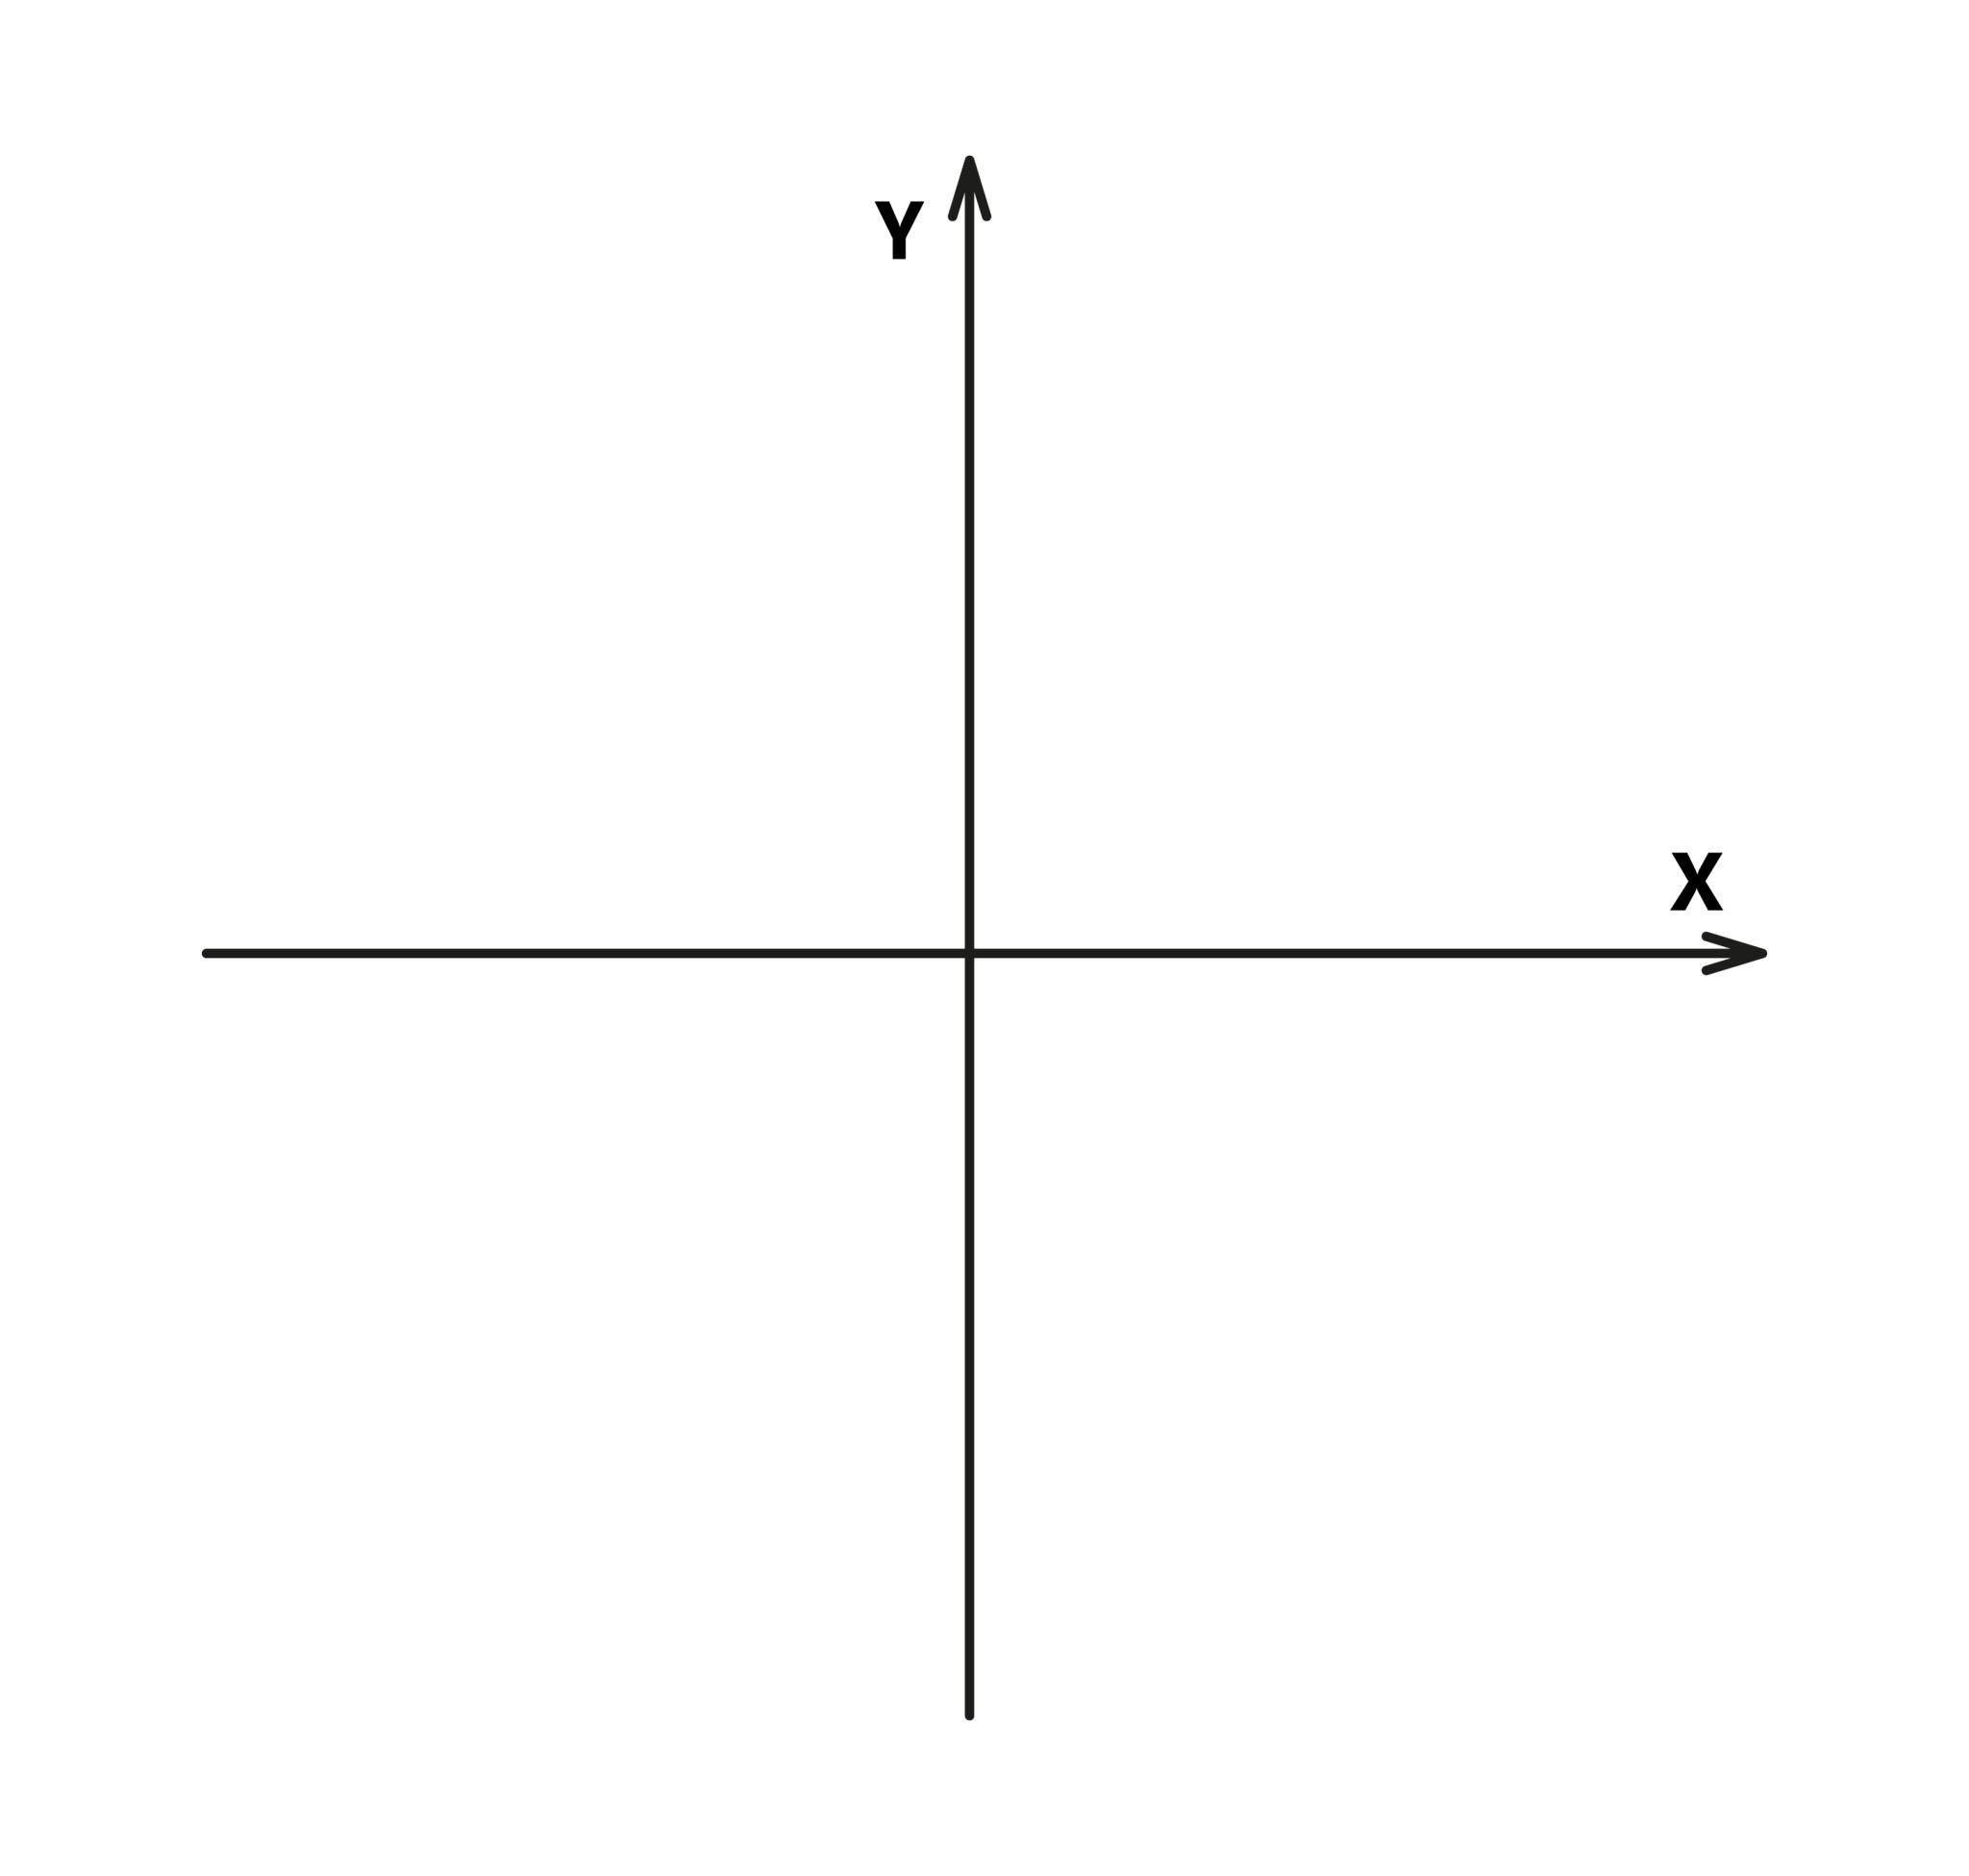
\includegraphics[width=\linewidth]{_graphic/graph-example.jpg}
          \end{figure}
    \end{minipage}
\end{frame}

\begin{frame}[label=section-anotherslide]{This is Another Slide}
    \begin{minipage}{0.49\linewidth}
        \begin{itemize}
            \item You can do the same with tables!
        \end{itemize}
    \end{minipage}
    \begin{minipage}{0.49\linewidth}
        \begin{table}[!tb]
            \centering
            \caption{Title}
            % \resizebox*{\textwidth}{!}{
            \begin{threeparttable}
                \small
                \begin{tabular}{lr}
    \toprule
    \multicolumn{1}{c}{Column 1} & \multicolumn{1}{c}{Column 2} \\ 
    \midrule
    Hello & World \\
    \bottomrule
\end{tabular}
                \begin{tablenotes}[flushleft]
                    \scriptsize{\item \textit{Notes}: This is a (short) note.}
                \end{tablenotes}
            \end{threeparttable}
            % }
        \end{table}
    \end{minipage}
\end{frame}